%!TEX program = xelate
%%%%%%%%%%%%%%%%%%%%%%%%%%%%%%%%%%%%%%%%%
% Modified By Orcuslc, 2016-9-21
% Modified for Assignments
% http://github.com/orcuslc
%
% Wilson Resume/CV
% Structure Specification File
% Version 1.0 (22/1/2015)
%
% This file has been downloaded from:
% http://www.LaTeXTemplates.com
%
% License:
% CC BY-NC-SA 3.0 (http://creativecommons.org/licenses/by-nc-sa/3.0/)
%
%%%%%%%%%%%%%%%%%%%%%%%%%%%%%%%%%%%%%%%%%

%----------------------------------------------------------------------------------------
%	PACKAGES AND OTHER DOCUMENT CONFIGURATIONS
%----------------------------------------------------------------------------------------
\documentclass[10pt]{article}

\usepackage{listings}
\usepackage{xcolor}
\usepackage{amsmath,amsthm,amssymb}
\usepackage{epstopdf}
\usepackage{graphicx}
\usepackage{clrscode3e}

\DeclareGraphicsExtensions{.eps,.ps,.jpg,.bmp}


\usepackage[a4paper, hmargin=25mm, vmargin=30mm, top=20mm]{geometry} % Use A4 paper and set margins

\usepackage{fancyhdr} % Customize the header and footer

\usepackage{lastpage} % Required for calculating the number of pages in the document

\usepackage{hyperref} % Colors for links, text and headings

\setcounter{secnumdepth}{0} % Suppress section numbering

%\usepackage[proportional,scaled=1.064]{erewhon} % Use the Erewhon font
%\usepackage[erewhon,vvarbb,bigdelims]{newtxmath} % Use the Erewhon font
\usepackage[utf8]{inputenc} % Required for inputting international characters
\usepackage[T1]{fontenc} % Output font encoding for international characters

\usepackage{fontspec} % Required for specification of custom fonts
\setmainfont[Path = ./fonts/,
Extension = .otf,
BoldFont = Erewhon-Bold,
ItalicFont = Erewhon-Italic,
BoldItalicFont = Erewhon-BoldItalic,
SmallCapsFeatures = {Letters = SmallCaps}
]{Erewhon-Regular}

\usepackage{color} % Required for custom colors
\definecolor{slateblue}{rgb}{0.17,0.22,0.34}

\usepackage{sectsty} % Allows customization of titles
\sectionfont{\color{slateblue}} % Color section titles

\fancypagestyle{plain}{\fancyhf{}\cfoot{\thepage\ of \pageref{LastPage}}} % Define a custom page style
\pagestyle{plain} % Use the custom page style through the document
\renewcommand{\headrulewidth}{0pt} % Disable the default header rule
\renewcommand{\footrulewidth}{0pt} % Disable the default footer rule

\setlength\parindent{0pt} % Stop paragraph indentation

% Non-indenting itemize
\newenvironment{itemize-noindent}
{\setlength{\leftmargini}{0em}\begin{itemize}}
{\end{itemize}}

% Text width for tabbing environments
\newlength{\smallertextwidth}
\setlength{\smallertextwidth}{\textwidth}
\addtolength{\smallertextwidth}{-2cm}

\newcommand{\sqbullet}{~\vrule height .8ex width .6ex depth -.05ex} % Custom square bullet point 


\newcommand{\tbf}[1]{\textbf{#1}}
\newcommand{\tit}[1]{\textit{#1}}
\newcommand{\mbb}[1]{\mathbb{#1}}
\newcommand{\blue}[1]{\color{blue}{#1}}
\newcommand{\red}[1]{\color{red}{#1}}
\newcommand{\sblue}[1]{\color{slateblue}{#1}}
\newcommand{\n}{\\[5pt]}
\newcommand{\tr}{^\top}
\newcommand{\vt}[1]{
\Vert #1 \Vert
}
\newcommand{\bra}[5]{
#1=\left\{
\begin{aligned}
#2 ,&\quad #4 \\
#3 ,&\quad #5
\end{aligned}
\right.
}

\renewcommand{\title}[2] {
{\Huge{\color{slateblue}\textbf{#1}}}
\hfill
\LARGE{\color{slateblue}\textbf{#2}} \\[10pt]
\large{\color{slateblue}\textbf{Chuan Lu, 13300180056, chuanlu13@fudan.edu.cn}} \\[1mm]
\rule{\textwidth}{0.5mm}
}

\newcommand{\problem}[2] {
\vspace{20pt}
\LARGE{\color{slateblue}\textbf{Problem #1.}}
\vspace{2mm}
#2 \\[10pt]
}

\renewcommand{\proof}[2] {
\large{\color{slateblue}\textit{\textbf{#1.}}}
#2 \qed \\[3mm]
}

\newcommand{\solution}[2] {
\large{\color{slateblue}\textit{\textbf{#1.}}}
#2 \\[3mm]
}


\newcommand{\algorithm}[2] {
\begin{codebox}
\Procname{$\proc{Algorithm #1}$}
#2
\end{codebox}
}

\newcommand{\refgroup}[1] {
\LARGE{\color{slateblue}\textbf{Reference}} 
\begin{tabbing}
\hspace{5mm} \= \kill
#1
\end{tabbing}
}

\newcommand{\reference}[1] {
\sqbullet \ \  \large{#1} \\
}
% \newcommand{\solution}[2] {
% \LARGE{\color{slateblue}\textit{#1}}
% \ #2 \qed
% }

% \newenvironment{problem}[2][Problem]{\begin{trivlist}
% \item[\hskip \labelsep {\bfseries #1}\hskip \labelsep {\bfseries #2.}]}{\end{trivlist}}
\usepackage{epstopdf}
\usepackage{graphics}
\usepackage{subfig}
\usepackage{listings}
\lstset{
  breaklines=true,
  xleftmargin=25pt,
  xrightmargin=25pt,
  aboveskip=0pt,
  belowskip=10pt,
  basicstyle=\ttfamily,
  showstringspaces=false,
  frame=ltrb,
  tabsize=4,
  numbers=left,
  numberstyle=\small,
  numbersep=8pt,
  morekeywords={*, factorial, sum, erlang},
  keywordstyle=\color{blue!70}, commentstyle=\color{red!50!green!50!blue!50},
}
\DeclareGraphicsExtensions{.eps,.ps,.jpg,.bmp}

\begin{document}

\title{Numerical Analysis \\ Assignment 8}
\date{\today}
\author{Chuan Lu}

\maketitle

\problem{1}{Problem 3.42, Page 193}
\solution{(a)}{
Consider
$$
e^{i\frac{2\pi jk}{m}} = \cos\left(\frac{2\pi jk}{m}\right) + i\sin\left(\frac{2\pi jk}{m}\right).
$$
Then if $k$ is a multiple of $m$, we have 
$$
\sum_{j=0}^{m-1}\cos\left(\frac{2\pi jk}{m}\right) = \sum_{j=0}^{m-1}1 = m.
$$
Otherwise we have
$$
\sum_{j=0}^{m-1}\cos\left(\frac{2\pi jk}{m}\right)+i\sum_{j=0}^{m-1}\sin\left(\frac{2\pi jk}{m}\right) = \sum_{j=0}^{m}e^{i\frac{2\pi jk}{m}} = \frac{1-e^{i\frac{2\pi k}{m}m}}{1-e^{i\frac{2\pi k}{m}}} = 0.
$$
Thus
$$
\sum_{j=0}^{m-1}\cos\left(\frac{2\pi jk}{m}\right) = \sum_{j=0}^{m-1}\sin\left(\frac{2\pi jk}{m}\right) = 0.
$$
}
\solution{(b)}{
$$
\sum_{j=0}^{m-1}\cos\left(\frac{2\pi jk}{m}\right)\cos\left(\frac{2\pi jl}{m}\right) = \frac{1}{2}\sum_{j=0}^{m-1}\left(\cos\left(\frac{2\pi j(k+l)}{m}\right) + \cos\left(\frac{2\pi j(k-l)}{m}\right)\right)
= \left\{
\begin{aligned}
&m, ~k=l=\frac{m}{2} \\
&\frac{m}{2}, ~k=l\ne\frac{m}{2}, ~\text{or}~ k+l = m, k\ne l\\
&0, ~\text{others}
\end{aligned}
\right.
$$
$$
\sum_{j=0}^{m-1}\sin\left(\frac{2\pi jk}{m}\right)\sin\left(\frac{2\pi jl}{m}\right) = \frac{1}{2}\sum_{j=0}^{m-1}\left(\cos\left(\frac{2\pi j(k-l)}{m}\right) - \cos\left(\frac{2\pi j(k+l)}{m}\right)\right)
= \left\{
\begin{aligned}
&\frac{m}{2}, ~k=l\ne\frac{m}{2}\\
&-\frac{m}{2}, ~k+l=m, k\ne l \\
&0, ~\text{others}
\end{aligned}
\right.
$$
$$
\sum_{j=0}^{m-1}\cos\left(\frac{2\pi jk}{m}\right)\sin\left(\frac{2\pi jl}{m}\right) = \frac{1}{2}\sum_{j=0}^{m-1}\left(\sin\left(\frac{2\pi j(k+l)}{m}\right) + \sin\left(\frac{2\pi j(l-k)}{m}\right)\right)
= 0.
$$
}

\problem{2}{Problem 3.43, Page 194}
\solution{(a)}{
$$
d_k = \frac{1}{m}\sum_{j=0}^{m-1}w_m^{jk}x_j = \frac{1}{m}\sum_{j=0}^{m-1}e^{-i\frac{2\pi jk}{m}}.
$$
The same with Problem 1, 
$$
d_k = \left\{
\begin{aligned}
&1, ~k=0 \\
&0, ~k\ne 0
\end{aligned}
\right.
$$
}
\solution{(b)}{
$$
d_k = \frac{1}{m}\sum_{j=0}^{m-1}w_m^{jk}x_j = \frac{1}{m}\sum_{j=0}^{m-1}(-1)^ke^{-i\frac{2\pi jk}{m}} = \frac{1}{m}\frac{1-(-1)^me^{-i2\pi jk}}{1-(-1)e^{-i\frac{2\pi k}{m}}} = 
\left\{
\begin{aligned}
&1, ~k = \frac{m}{2}, ~m = 2n \\
&0, ~\text{other}~ k, ~m = 2n \\
\end{aligned}
\right.
$$
}
\solution{(c)}{
$$
d_k = \frac{1}{m}\sum_{j=0}^{m-1}je^{-i\frac{2\pi jk}{m}} = \frac{1}{e^{-i\frac{2\pi k}{m}}-1}((m-1)e^{-i2\pi k}-\frac{e^{-i\frac{2\pi k}{m}}(1-e^{-i2\pi k})}{1-e^\frac{-i2\pi k}{m}}) = 
\left\{
\begin{aligned}
&\frac{m-1}{2}, ~k=0 \\
&\frac{m-1}{e^{-i\frac{2\pi k}{m}}-1}, ~k\ne 0
\end{aligned}
\right.
$$
}

\problem{3}{ Consider approximating $f(x) = e^{\sin(x)}$ on $[0, 2\pi]$, using the triogometric interpolation $P_n(t)$. Create an maximum error  table for $n=1, \cdots,n$.}
\lstinputlisting{trigonometric.m}
\lstinputlisting{main.m}
\begin{lstlisting}[language = MATLAB]
>> error

error =

    1.7183
    1.7183
    0.3823
    0.4854
    0.2799
    0.1285
\end{lstlisting}
\begin{figure}[!htb]
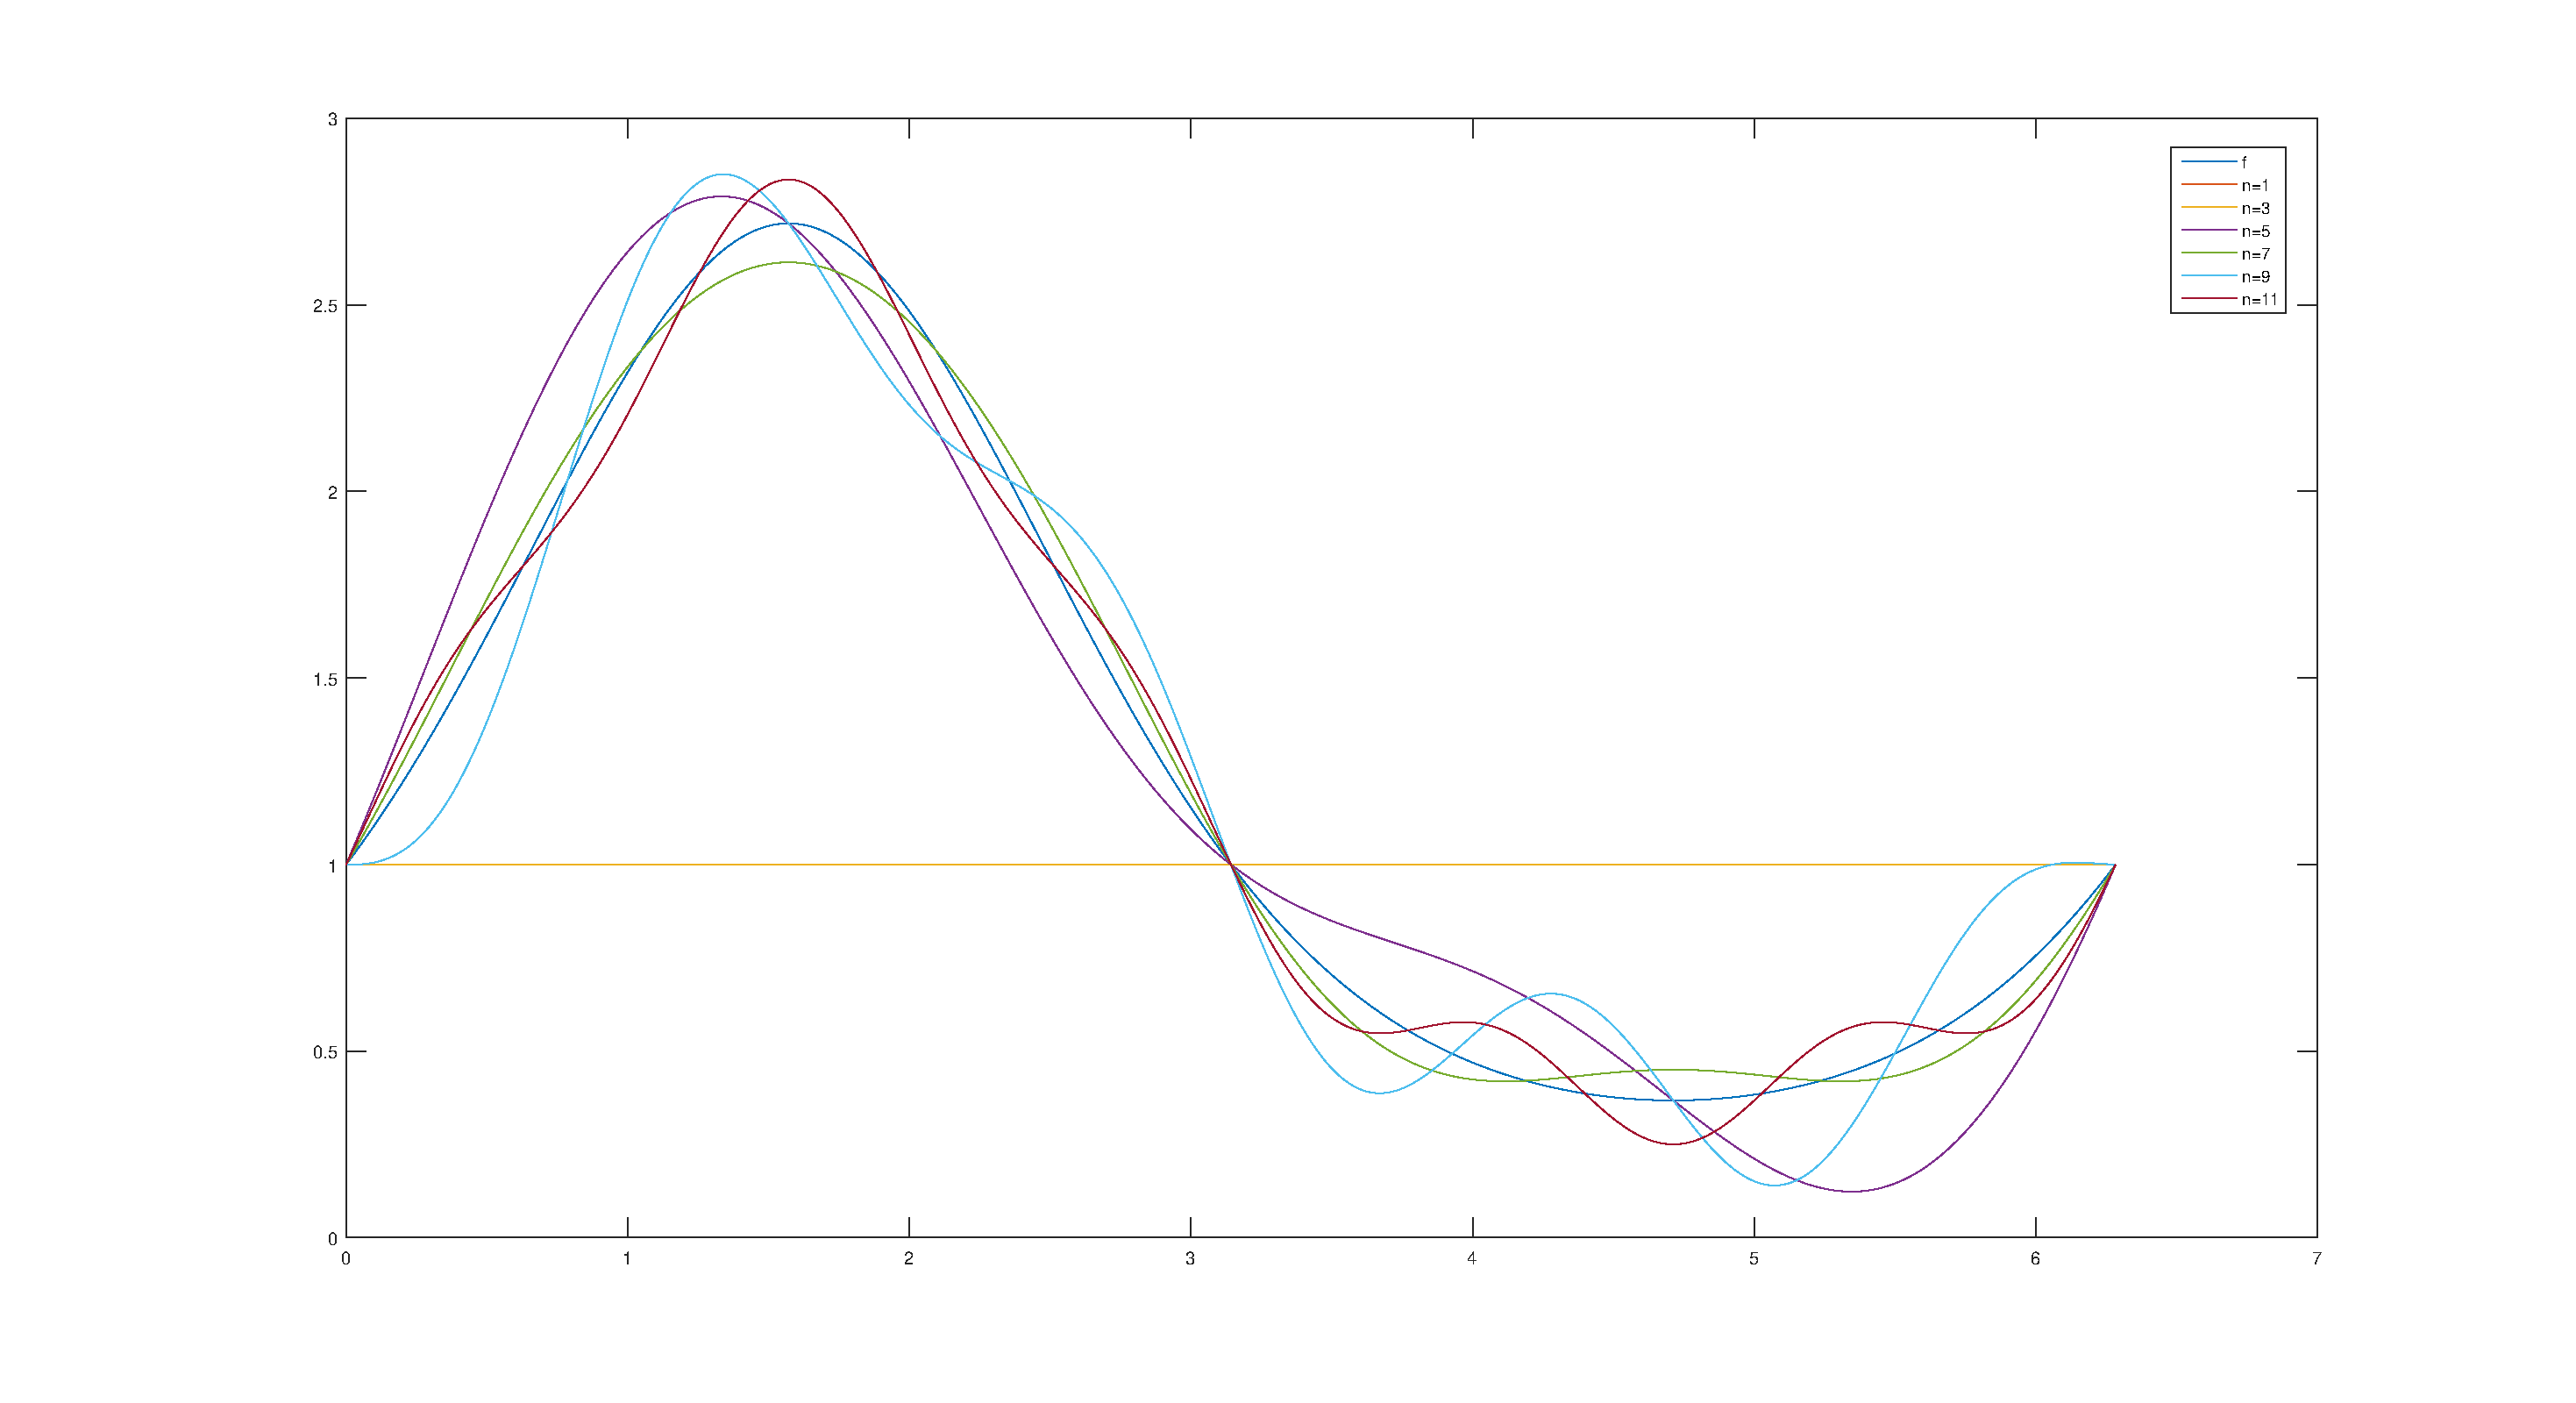
\includegraphics[width = \textwidth]{res.eps}
\end{figure}
\end{document}